\section{Aplicación web}

Como se muestra en la Figura \ref{fig:procesoAppWeb}, la aplicación web desarrollada consta de 7 etapas, este proceso se llevará a cabo la primera vez que se seleccione una sección o en el caso de que hayan transucurrido 4 horas de la última vez que se utilizó el sistema.
\\

\begin{figure}[H]
	\centering
	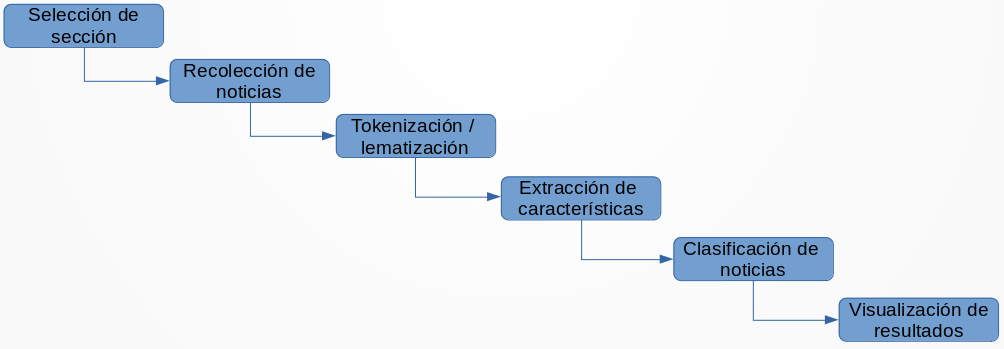
\includegraphics[scale=0.3]{imagenes/Capitulo5/procesoRecoleccionClasificacion.png}
	\caption{Etapas de la aplicación web}
	\label{fig:procesoAppWeb}
\end{figure}

\subsubsection{Selección de sección}
El usuario tendrá que elegir una sección (Cultura, Deportes, Economía, Política o Ciencia y Tecnología). 
\\

\subsubsection{Recolección de noticias}
Una vez seleccionada la sección, se procede con la recolección de noticias de los sitios web previamente definidos, la información que se descargará de cada noticia será la siguiente:

\begin{itemize}
	\item URL de la noticia
	\item Título
	\item Fecha
	\item Autor
	\item Descripción \footnote{Existen sitios web, donde las noticias cuentan con una descripción}
	\item Noticia
\end{itemize}

No será necesario extraer el nombre de la sección a la cual pertenece la noticia.\\

\subsubsection{Tokenización / lematización}
Una vez que el contenido de las noticias, pasan por la etapa de tokenización, la cual consiste en separar el texto en sus elementos mínimos, posteriormente se procese con la lematización del texto, proceso que reduce cada una de las palabras tokenizadas en lemas.


\subsubsection{Extracción de características}
Finalizado el proceso de tokenización y lematización, se procede con la etapa de extracción de características, donde se crea un espacio vectorial por cada noticia, en donde cada elemento del vector representa la existencia o asencia de una característica (palabra).

\subsubsection{Clasificación de noticias}
Una vez que se han obtenido las características de cada una de las noticias, se realizá la clasificación de las noticias, estas noticias se guardarán en un archivo, cabe destacar que cada sección contendrá su propio archivo, con el fin de mejorar el tiempo de visualización de los resultados.

\subsubsection{Visualización de resultados}
El usuario podrá visualizar las noticias extraídas y clasificadas de la sección que seleccione, 

\subsection{Vistas de la aplicación web}

El sistema cuenta con 5 secciones Deportes, Economía, Política, Cultura y Ciencia y tecnología, el usuario podrá elegir de alguna de estas secciones, se debe considerar que los sitios web de los cuales serán recolectadas las noticias, han sido definidos en el caítulo 5.1.\\
La Figura \ref{fig:PantallaInicio} muestra la vista que tendrá el usuario al ingresar a la aplicación web
\\
\begin{figure}[H]
\centering

\includegraphics[scale=0.29]{imagenes/Capitulo5/pantallaPrincipal.png}
\caption{Pantalla de Inicio.}
\label{fig:PantallaInicio}
\end{figure}

El usuario tiene la posibilidad de elegir la sección de la cual desee visualizar noticias. Una vez que el usuario seleccione una sección, la vista que tendrá se muestra en la Figura \ref{fig:loading}.
\\
\begin{figure}[H]
\centering
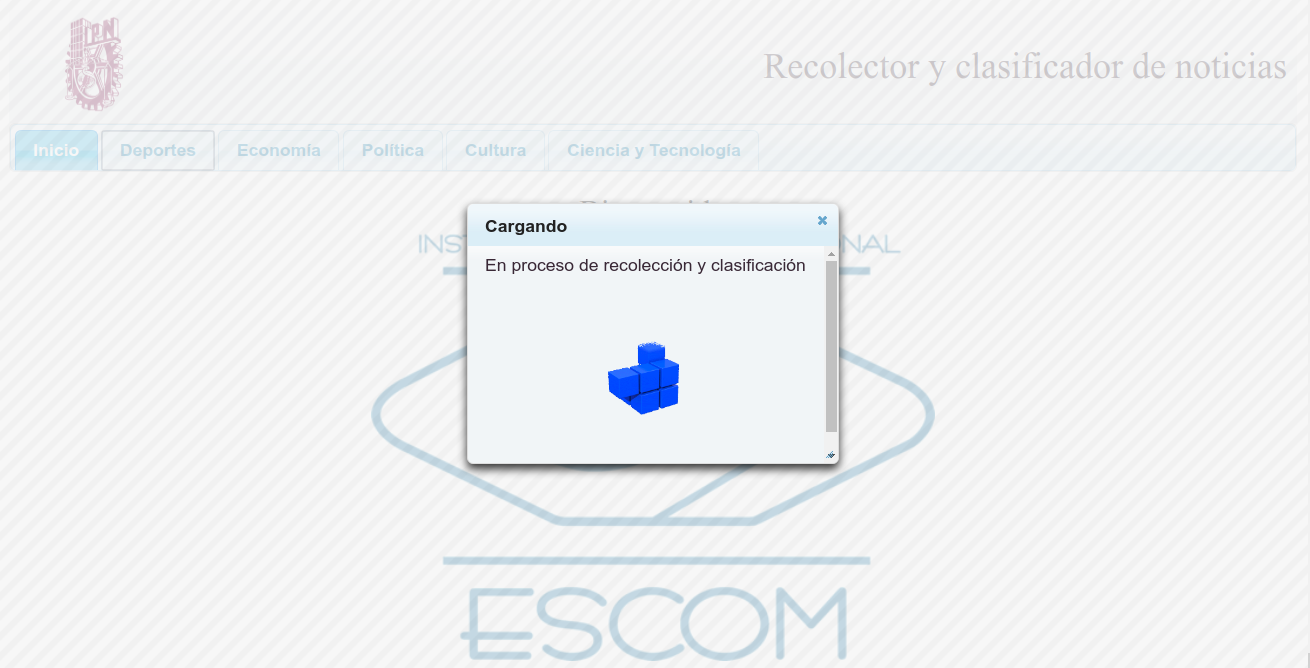
\includegraphics[scale=0.29]{imagenes/Capitulo5/mensajeEspera.png}
\caption{Mensaje de espera.}
\label{fig:loading}
\end{figure}

Mientras se muestra esta vista, de manera interna se realizan los siguientes procesos:

\begin{itemize}
	\item Se realiza la recolección de noticias.  
	\item Una vez finalizada la recolección de noticias, se unen en un archivo
	\item Se tokenizan y lematizan las noticias recolectadas
	\item Finalmente el algoritmo clasifica las noticias recolectadas
\end{itemize}

Una vez que se han clasificado las noticias el usuario tendrá la opción de elegir si desea visualizar las noticias o cancelar, la Figura \ref{fig:notClass}, muestra el mensaje que el usuario visualizará una vez finalizada la clasificación.
\\
\begin{figure}[H]
\centering
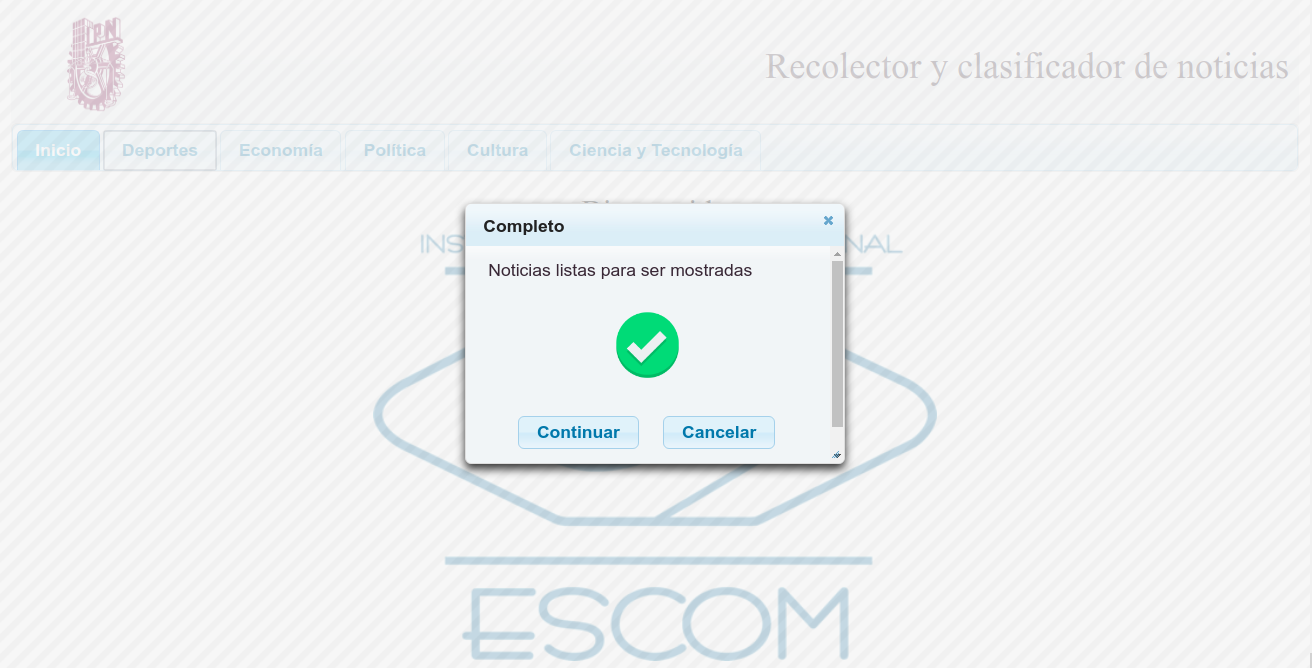
\includegraphics[scale=0.29]{imagenes/Capitulo5/noticiasListasParaSerMostradas.png}
\caption{Mensaje que se muestra una vez clasificadas las noticias.}
\label{fig:notClass}
\end{figure}

Las noticias se mostrarán por fecha de publicación, mostrándose las del día actual, en la pantalla principal, la información que se mostrará será el título de la noticia, el resúmen de la noticia si es que tiene, el autor de la noticia y finalmente la fecha de publicación de la noticia.\\
Si el usuario selecciona continuar, la vista que tendrá el usuario se muestra en la Figura \ref{fig:vistaNoticias}.
\\
\begin{figure}[H]
\centering
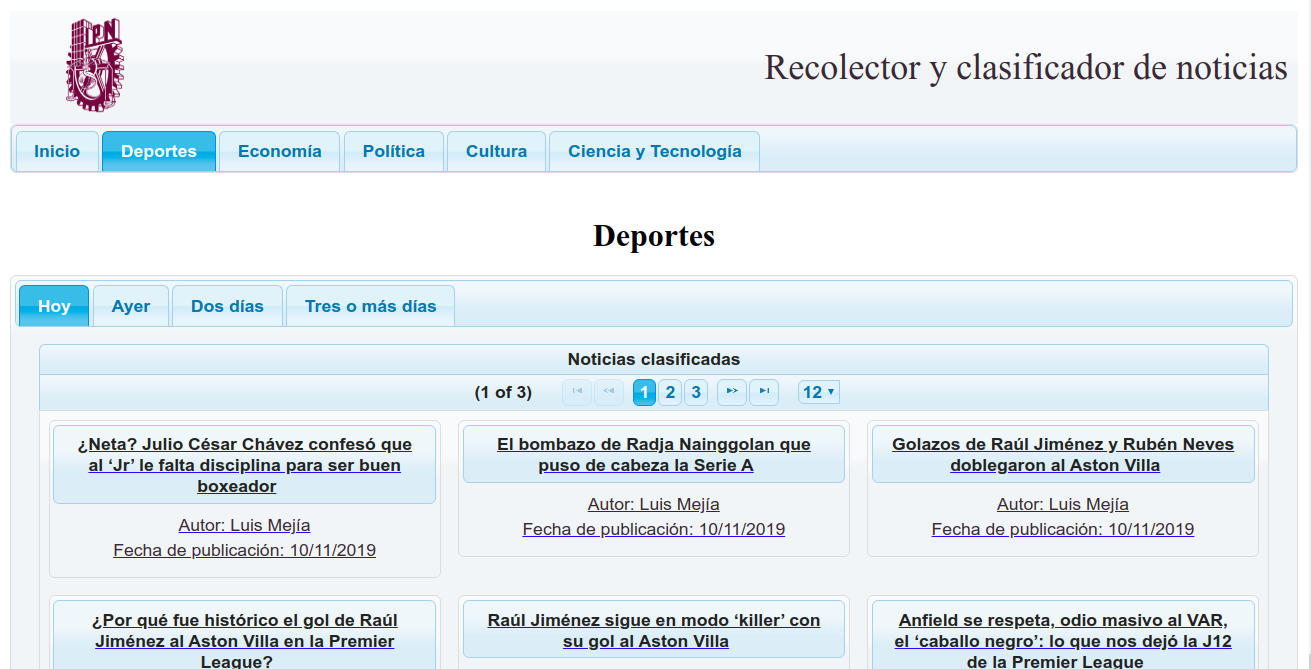
\includegraphics[scale=0.29]{imagenes/Capitulo5/noticiasDeHoy.png}
\caption{Vista de las noticias recolectadas.}
\label{fig:vistaNoticias}
\end{figure}

Si el usuario desea visualizar noticias del dia de ayer, la vista que tendrá se muestra en la Figura \ref{fig:vistaNoticiasAyer}.
\\
\begin{figure}[H]
\centering
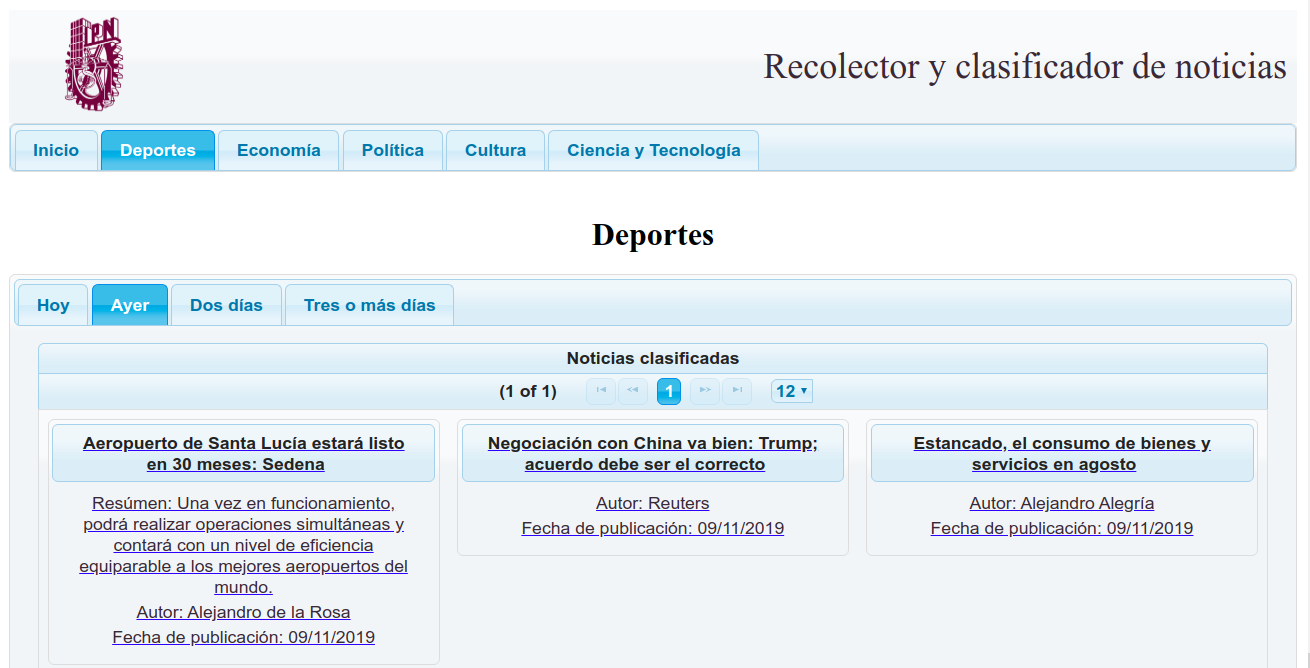
\includegraphics[scale=0.29]{imagenes/Capitulo5/noticiasDeAyer.png}
\caption{Vista de las noticias recolectadas del día de ayer.}
\label{fig:vistaNoticiasAyer}
\end{figure}

Existe la posibilidad de que no se recolecten noticias, si después de 84 segundos, no se realizó la recolección de noticias debido a una falla con nuestra conectividad de Internet, la pantalla que el usuarió tendrá se muestra en la Figura \ref{fig:notNoRec}.
\\
\begin{figure}[H]
\centering
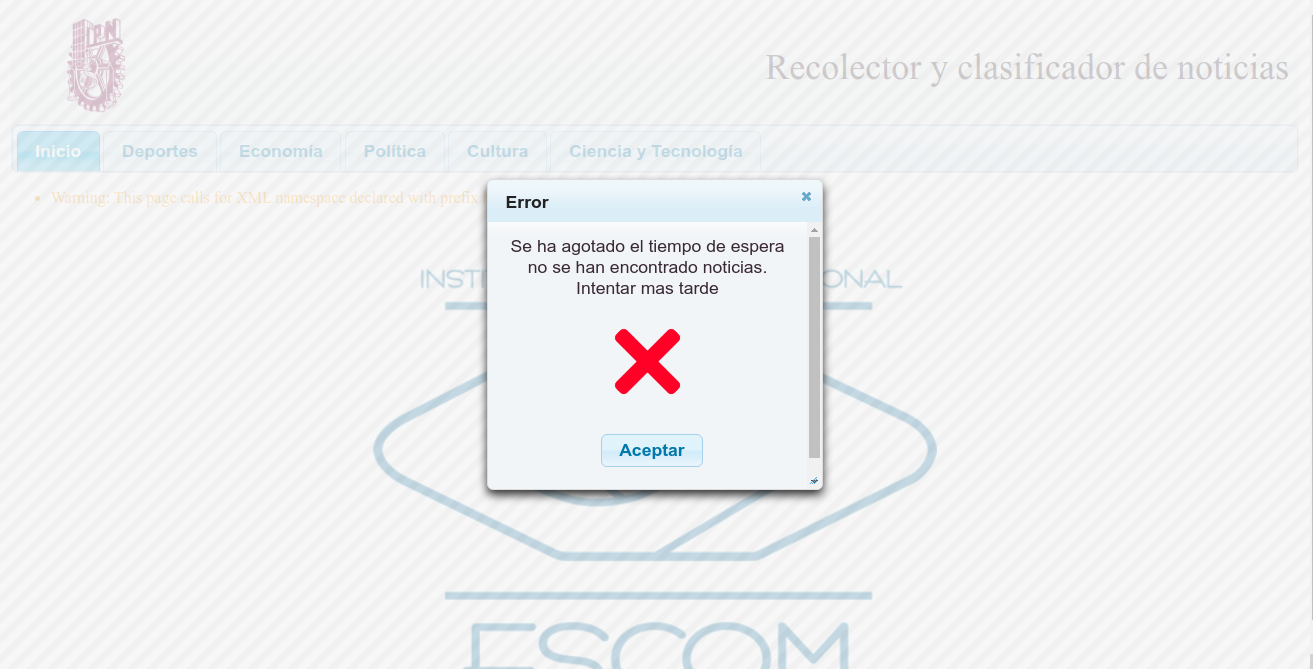
\includegraphics[scale=0.29]{imagenes/Capitulo5/errorConectividad.png}
\caption{Mensaje que se muestra si no se recolectaron noticias.}
\label{fig:notNoRec}
\end{figure}

